
\documentclass{article}
\usepackage{graphicx} % Required for inserting images
\usepackage{listings} % Required for displaying code
\usepackage{float}


\title{Project 2}
\date{April 28, 2023}
\begin{document}  


\maketitle
\noindent We have {\bf read and understood the assignment instructions}. We certify that the submitted work does not violate any academic misconduct rules, and that it is solely our own work. By listing our names below we acknowledge that any misconduct will result in appropriate consequences. 

\vspace{0.2in}

\noindent {\em ``As a Boilermaker pursuing academic excellence, I pledge to be honest and true in all that I do.
Accountable together -- we are Purdue.''}

\vspace{0.3in}

\begin{table}[h!]
  \begin{center}
    \label{tab:table1}
     \begin{tabular}{c|ccccc|c|c}
      Student & Sub-Algorithm 1-5 & Main Algorithm  & Report & Overall & DIFF\\
      \hline
      Chirayu Marwaha & 20 & 20  & 20 & 100 & 0\\
      Liz Parmenter & 20 & 20  & 20 & 100 & 0\\
      Abdulla Almarzooqi & 20  & 20 & 20 & 100 & 0\\
      Hongyi Shen & 20 & 20 & 20 & 100 & 0\\
      Kevin Braner & 20 & 20 & 20 & 100 & 0\\
      \hline
      St Dev & 0 & 0 & 0 & 0 & 0 
    \end{tabular}
  \end{center}
\end{table}
\newpage
\section{Introduction}
In this project, we have created 5 sub-algorithms that perform adversarial attacks on the given image classifier. These sub algorithms run within our main algorithm that assigns weight to images. From this, our algorithm will fool the given image classifier. We have done this by changing 1 percent of the available pixels. The images we were given have differing numbers of pixels so we took this into account. We completed the IE 332 Spring 2023 Project 2 between the months of April and May with semi-success by using time management and commitment to the project objectives. In this report we will discuss algorithm and decision classifier choices, implementation, and completed plans. The project showcases the application of IE 332 knowledge to manage and understand data using computers in the real world.

\section{Methods}
\subsection{RGB Pixel Swap}
In the first sub-algorithm, the code loads the necessary packages. It then sets the working directory and loads the pre-trained machine learning model from a saved file. Finally the model's summary is printed. The random function is defined to modify the input images by changing a certain percentage of pixels in the image. Specifically, it modifies the RGB values of a pixel to yellow (red=1, green=1, blue=0). The modified image is saved as a JPEG file and then reloaded using read JPEG. The code then loops through a folder containing images of grass and dandelions, loads each image, reprocesses the image and sets scaling pixel values to be between 0 and 1, modifies the image using random function, pre-processes the modified image, and then predicts the class of the image using the pre-trained model with predict. The predicted probabilities for each class are printed using print. The loop is run twice, once for grass images and once for dandelion images. Finally, the code loops through the same folders again but this time does not modify the images before predicting their class using the pre-trained model. The predicted probabilities for each class are printed using print.


\subsection{Square Contrasting Color Overlay}
The square contrasting color overlay algorithm is designed to fool the classifier by inserting a square of constant color pixels in the center of the image. The algorithm loops through images in the specified folder, and performs a single prediction using the model to determine the classification of the inputs. If the inputs are classified as grass, a yellow square is produced. If the inputs are classified as dandelions, a yellow square is produced. These color selections were made based off visual observations of the sample images, which suggested that dandelions appeared to have a higher concentration of yellow pixels towards the center of the image, and vice versa for grass. \\
Next, the algorithm calculates the dimensions of the image, and uses these values to determine the largest square dimension using less than 1\% of the pixels, as shown in the following equation, where height and width refer to image dimensions:
\begin{equation} \label{eqn}
    L = floor(\sqrt{height * width * 0.01})
\end{equation}
This value is used to create an offset range where pixels are modified. The range calculations are shown below:
\begin{equation} \label{eqn}
    X Indices = (width/2 - L/2, width/2 + L/2)
\end{equation}

\begin{equation} \label{eqn}
    Y Indices = (height/2 - L/2, height/2 + L/2)
\end{equation}
Then, these selected indices' color channels are modified to produce either a green square (dandelions), or a yellow square (grass) as shown:

\begin{figure}
\centering
    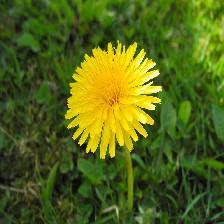
\includegraphics[scale = 0.5]{dandelion_constant.jpg}
    \caption{Original Dandelion image}
    \label{fig:my_label}
    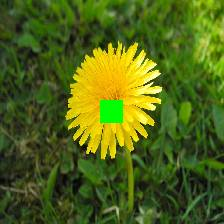
\includegraphics[scale = 0.5]{dandelion_constant_pert.jpg}
    \caption{Perturbed Dandelion image}
    \label{fig:my_label}
    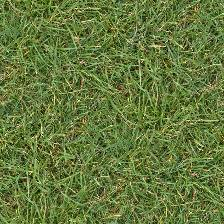
\includegraphics[scale = 0.5]{grass_constant.jpg}
    \caption{Original Grass image}
    \label{fig:my_label}
    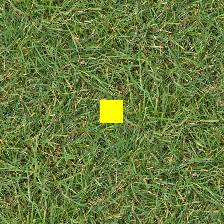
\includegraphics[scale = 0.5]{grass_constant_pert.jpg}
    \caption{Perturbed Grass image}
    \label{fig:my_label}
\end{figure}

This algorithm is very simple as it produced a nearly constant overlay for each image, and it used in contrast to some of the other algorithms which target specific color pixels or pixel intensity. It also is very easy to show that the algorithm only alters one percent of pixels due to the simple geometry of the modification. The testing, complexity, and performance of the algorithm will be further discussed in the appendix.

\subsection{Yellow - Green Pixel Shift}
\vspace{0.1in}
This Yellow - Green Pixel Algorithm aims to eliminate the color characteristics of each picture. As for dandelions images, it will first load the image package, and using a loop to import those images, to fast the operation time, it then resizes each picture into 224*224 pixels, and then, is does the operation that replacing the 1 percent pixels which has the highest red values into green. The detailed method of this is by first setting a threshold for the 1 percent pixels with the highest red values, and later setting their blue channel to 1, red and green to 0 (0, 0, 1). It shifts yellow pixels into green pixels. By this operation, the large areas on the follower will be replaces by green pixels, which would fool the model for recognizing the flower into grass. 
\vspace{0.15in}
\\For grass pictures, it does right the opposite. It replaces the 1 percent bluest pixels into red. By doing this, it will create yellow areas in the picture. Which will fool the model to recognize the dandelion flowers. 
\vspace{0.2in}
\\The algorithm works particularly well for dandelion pictures that has less area of yellow flower. It will fill the yellow flower with green pixels to make the model do the wrong judgement to classify it into grass area.
\begin{center}
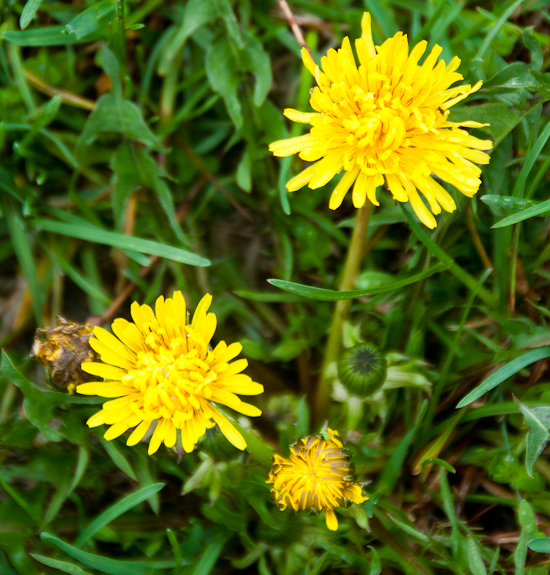
\includegraphics[scale=0.781]{dandelion-flowers-3932258560.jpg}\hspace{25pt}
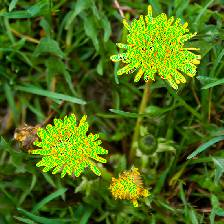
\includegraphics[scale=0.6]{thumbnail_image_11.jpg}\\
\hspace{2pt}Original Dandelion picture 
\hspace{30pt} Perturbed Dandelion picture
\end{center}
\vspace{0.2in}
\
Also, the algorithm works well for grass picture with flowers. The model will mistakenly classify the white flowers into dandelion flowers.
\begin{center}
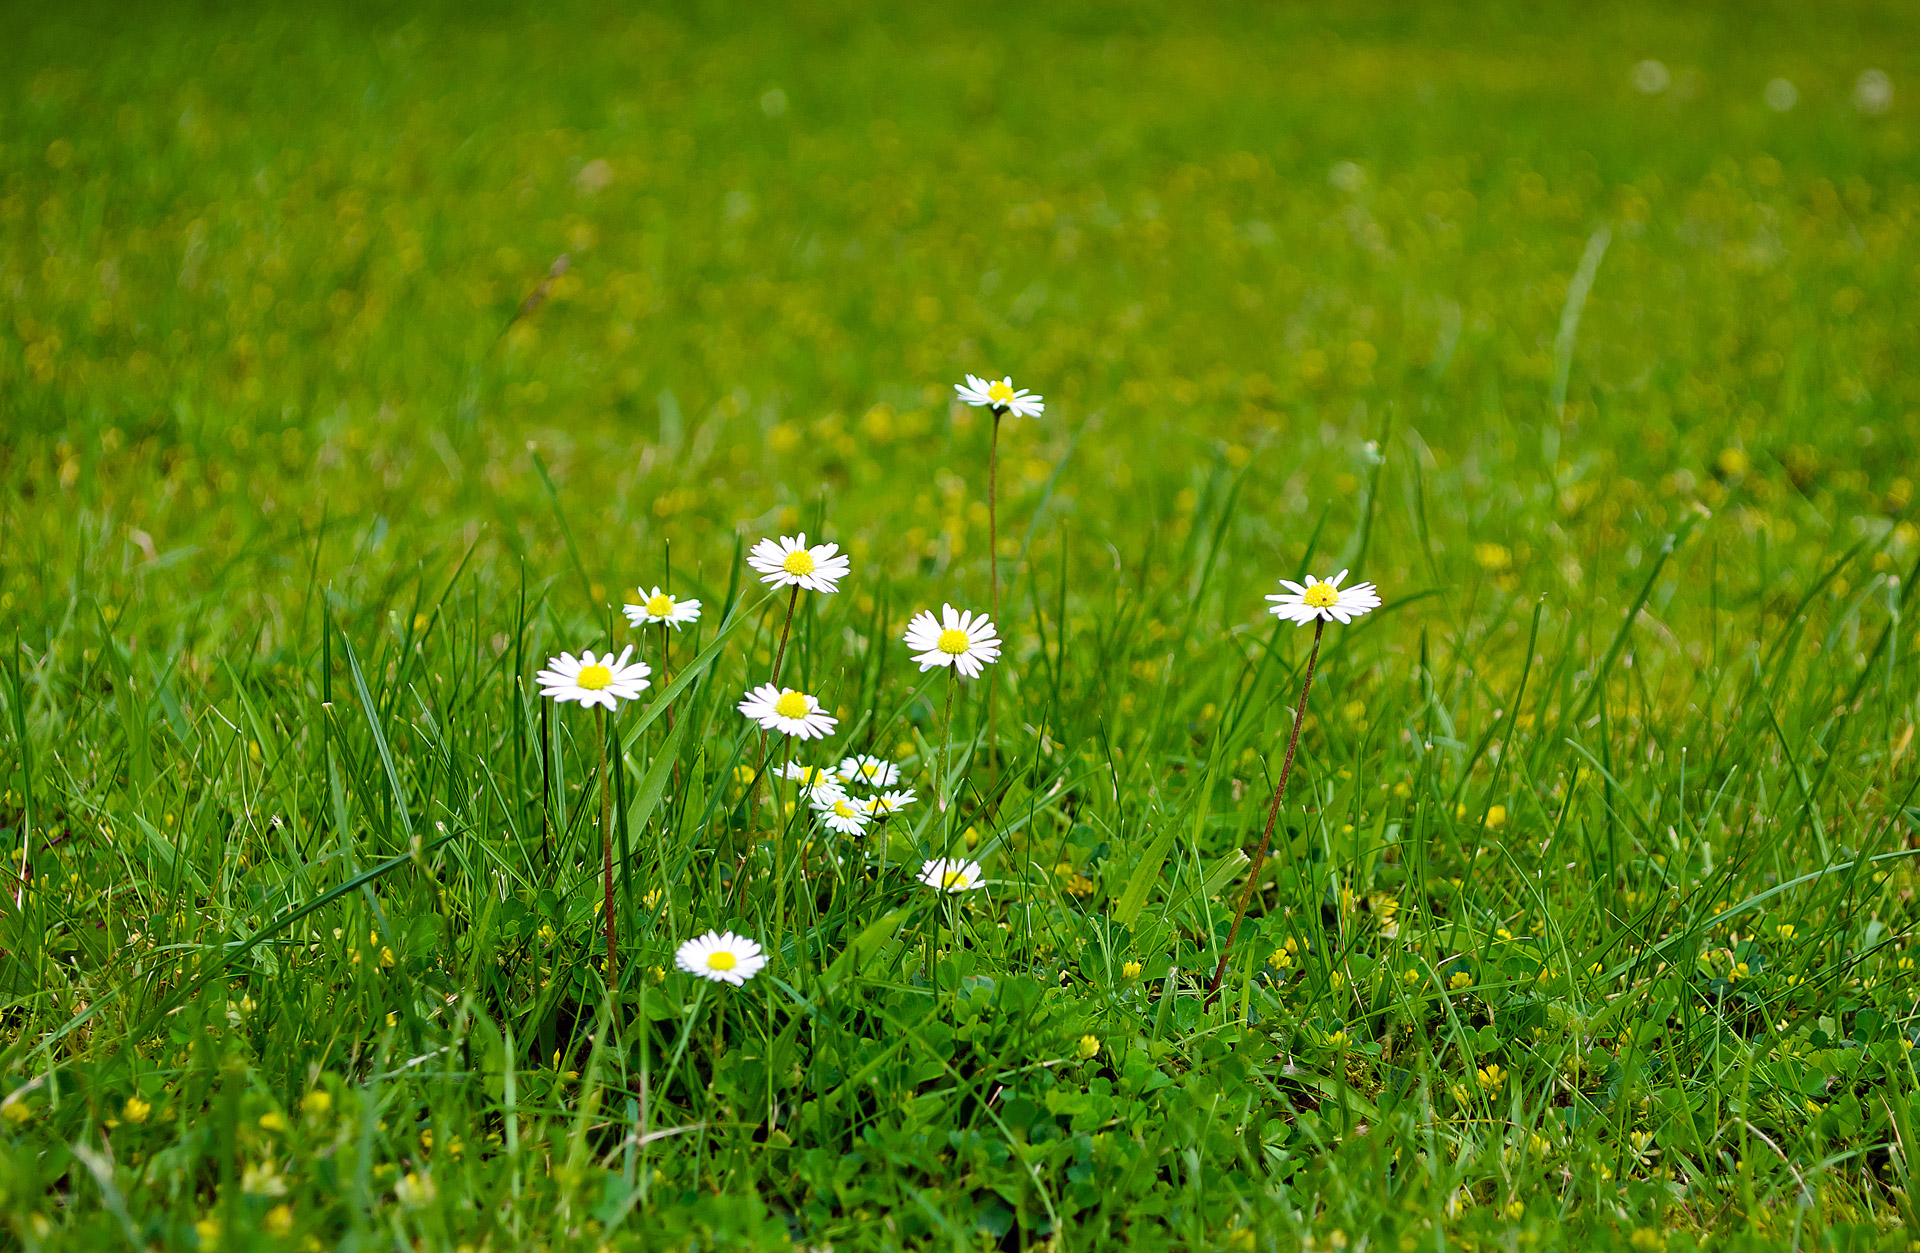
\includegraphics[scale=0.08]{flowers-on-the-grass-579853868.jpg} \hspace{15pt}
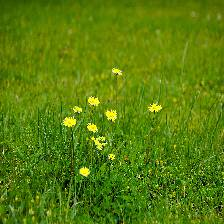
\includegraphics[scale=0.5]{thumbnail_image_13.jpg}\\
\hspace{25pt}Original Grass picture 
\hspace{45pt} Perturbed Grass picture\
\end{center}
\vspace{0.1in}
However, since the maximum pixel changing limit is only one percent of the total images, when facing dandelion which has bigger areas of flower, only a small area of it will be covered. And when facing grass images, since the changed areas does not has flower shaped, but more often the tips of the grass, or leaves lying on the grass, therefore, for dandelions with more yellow areas, or common grass images, it does not have a very high success rate. But at the same time, the simplicity for this algorithm, and the short running time of it, makes it a good choice in some situation. 

\subsection{CCP Attack}
The Color Channel Perturbation Attack (CCP Attack) is a type of adversarial attack on machine learning models that are trained on images. The goal of this attack is to modify the colors of an image in a way that is imperceptible to humans, but can cause the machine learning model to misclassify the image.

The methodology behind the attack is to target the color channels of the image, such as red, green, and blue. The modifications are done by adding a small amount of noise to each channel, or by shifting the values of each channel by a small amount. 

Machine learning algorithms rely heavily on color information when making predictions on images. By perturbing the color channels of an image, the attack will introduce subtle changes that can fool the machine learning algorithm into making incorrect predictions.

The perturbations generate the new transformed color channels; transformed red $(R^T)$, transformed green $(G^T)$, and transformed blue $(B^T)$, of the transformed image $(I^T)$. In essence, each one of $R^T$, $G^T$, and $B^T$ is the weighted combination of R, G, and B given as: 
$$R^T = s * (\frac{\alpha^r_i * R_i + \alpha^g_i * G_i + \alpha^b_i * B_i}{3}) + b$$
$$G^T = s * (\frac{\beta^r_i * R_i + \beta^g_i * G_i + \beta^b_i * B_i}{3}) + b$$
$$B^T = s * (\frac{\lambda^r_i * R_i + \lambda^g_i * G_i + \lambda^b_i * B_i}{3}) + b$$
\\
where s is a scale factor hyper-parameter - the parameter that controls the overall magnitude of the weight values in the neural network - b is the bias hyper-parameter - the parameter that determines how much input to a neuron needs to be shifted before being passed through an activation function - ${R, G, B} \in \mathbb{R}$ of the $i^th$ input image. $R^T_i, G^T_i, B^T_i$ are the intensity values in Red, Green, and blue channels of the transformed image $I^T_i$.
\\

\subsection{Image Overlay}
The Image Overlay algorithm was designed to fool the model by using a transparent image overlay of the wrong image. For example, in a grass image would have an altered image with a dandelion being placed over it. It would be transparent enough that is does not completely overshadow the grass but is just visible enough to fool the model. 

The algorithm works referencing the grass directory. From there, a list is formed and each individual image will be re-scaled to a 224x224 image for faster run times. The adversarial dandelion image, which will be used on all grass pictures, will also be of the same size. From there the algorithm will iterate through all images to be re-scaled and place the dandelion image over the collection of grass photos. The outputs would be placed into their individual output folders to be placed through the model. The same process takes place for the dandelions only to be overlaid with a photo of grass. 

As the model uses colors to differentiate images, altering the image itself with the wrong set of colors should confuse the algorithm in theory.

\subsection{Weighted Majority Algorithm (Main) (Attempt)}
The majority weighted classifier functions by first passing the input image into the 5 sub-algorithms. The sub-algorithms will each select the 1\% of pixels they would like to perturb, which constitute as "votes" weighted by the corresponding sub-algorithm. The pixels with the greatest number of votes are deemed the best candidates to perturb, and the algorithm ensures 1\% or less of pixels are selected. The output of the the weighted majority algorithm should be an image that fools the classifier.
\\
\\
To be more detailed, in the process of the single image, the main algorithm will call five sub-algorithm with the input of the picture path, and they will return the array of the location of their changed pixels. The main algorithm will then assign "weight" to the output for each sub-algorithm. The weight is determined by the success rate for different algorithms. The main algorithm will assign a bigger weight to an algorithm that has a higher success rate. For example, more weight will be assigned to an output with a 25\% successful rate compared to a 15\% output.    
\\
\\
The success rates can be obtained in the "performance" section.
\\
\\
A higher-weighted sub-algorithm will get more votes for its pixels output, and the main algorithm will select 1\% pixels that have the highest "votes", and it will output the final result by changing those pixels. 

\section{Results}
\subsection{RGB Pixel Swap}
This code should take into account the number of pixels per image. Based on this, a percent of pixels should be changed to RGB. The computer should then misclassify the image based on the results. I ran into a few errors running the code so I was not able to determine exactly how many pixels should be changed. With that in mind, I was also unable to determine the probability of images fooled. 

\subsection{Square Contrasting Color Overlay}
In testing, the algorithm was ran against every image in the given grass and dandelion folder, and outputted the perturbed images into separate folders. It also records any image paths where the algorithm mis-classified the image. The algorithm was then refactored to merge with the weighted majority classifier, such that the selected pixel locations are outputted as well, which constitute as votes.

\subsection{Yellow - Green Pixel Shift}
\vspace{0.1in}
The Yellow - Green pixel Shift method will create a new folder that contain the perturbed images. In order to test the perturbed imaged weather they can fool the model classifier, We used the testing model to run through the generated model to check if the probability fall under 50 percent. if the percentage is less than 50 percent, it means the image successfully fooled the model. This process could be shown as follows:
\begin{center}
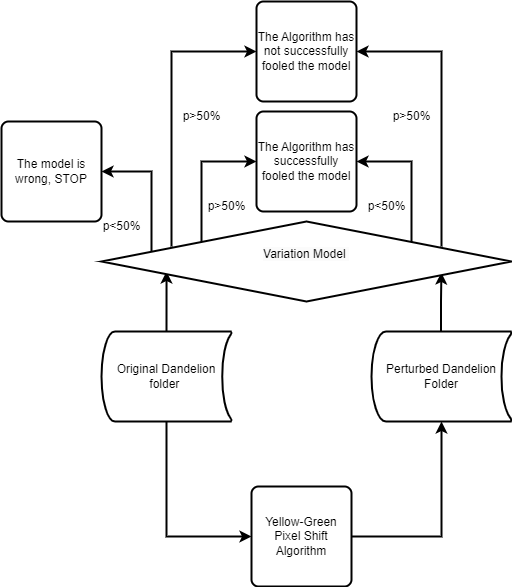
\includegraphics[scale = 0.5]{YGS_1.drawio.png}
\end{center}
The result is presented as follows:
\\
\subsection{CCP Attack}
In the context of this project, the CCP Attack was implemented in two functions, "change-brightness", and "CCP-Atk-Bright." The change-brightness function takes an image parameter which is expected to be a 2D or 3D array of pixel values representing the image. The alpha parameter in the function is a scalar value used to adjust the image's brightness, while the beta parameter adjusts the contrast. A new image is initialized as a zero array with the same dimensions as the input image. Using the 'pmax' function, the pixel values of the new image are set such that they are scaled by alpha and shifted by beta. Any pixel value less than zero are set to zero, and any pixel value higher than 225 are set to 225. The output of the function is the new image with adjusted brightness and contrast.
\\
\\
The CCP-Atk-Bright function takes two input parameters, image and trans. The image parameter is expected to be a 3D array of pixel values representing an RGB image. The trans parameter is a 3x3 matrix used to perform color correction transform on the image. The function first begins by creating a copy of the input image and assigns it to variable 'img.' It then loops over each color channel in the image and performs the color correction transformation on each channel individually. The color correction transform is performed by multiplying the pixel values of each channel by the corresponding row of the 'trans' matrix, and generates the sum of the results across all three rows. After the color correction transform is applied to each channel, the function computes the average of the resulting values across the three color channels to produce a grey-scale version of the image. This grey-scale version of the image is passed as the 'image' argument to the 'change-brightness' function, with parameters alpha = 1 and beta = 30. The 'change-brightness' function then returns a new image withe same dimensions as the input image, where the pixel values have been adjusted to increase the overall brightness of the image by adding 30 to each pixel value. 'CCP-Atk-Bright' then returns the new, brightened image. 
\subsection{Image Overlay}

The Image Overlay algorithm will create two respective folders with the updated images. Which serve the purpose of being inputted within the model to be run through. It is anticipated that the presence of contradicting colors will confuse the algorithm to answer incorrectly with confidence. 

\subsection{Weighted Majority Algorithm}
Unfortunately, we were unable to get the weighted majority algorithm to produce a perturbed image, as coordinating the inputs and outputs of the sub-algorithms proved to be a challenge in the limited time frame we had. The attempt at the weighted majority algorithm can be found under the branch "KevinBraner-WeightedMajorityClassifier".

\section{Challenges}
We ran into a variety of challenges during this project. First, there were a lot of Tensorflow documentation in Python which made it much more of a challenge to use in R. Another issue we ran into was accessing some of the libraries. We had to revert to Jupiter notebook to utilize some of them and it was not a very efficient process. Additionally, while designing the weighted majority classifier, we realized that we had discrepancies between the inputs and outputs of our sub-algorithms, which made them difficult to integrate. This was likely the result of version control mistakes, as it was the first time using Git for most of the group. Viewing existing branches and modeling new sub-algorithms off of the method signatures of existing sub-algorithms could have relieved this issue.


\section{Conclusion}
Throughout this project, we created 5 sub algorithms to perform adversarial attacks on an image classifier. These sub-algorithms are run within a main algorithm that assigns weight to images. The RGB Pixel Swap algorithm modifies input images by changing a certain percentage of pixels in the image to red green and blue. The Square Contrasting Color Overlay algorithm inserts a square of constant color pixels in the center of the image to produce either a green square (dandelions) or a yellow square (grass). The Yellow-Green Pixel Shift algorithm aims to eliminate the color characteristics of each picture. It replaces the 1 percent of pixels with the highest red values into green for dandelions and replaces the 1 percent blue pixels into red for grass pictures. The CCP Attack algorithm targets the three color channels of the input image by first scaling the pixel of the images to certain parameters, then changing the values of the pixels by 30 to increase the brightness of the input image. The resulting image should have higher pixel values intended to fool the binary image classifier model. The Image Overlay algorithm attempted to place a different image to fool the model. By placing a picture of dandelions over the grass, the hope was to fool the model by mistaking it for the other image. The same concept was applied to images of grass which were to be overlapped by an image of dandelions.

This project aims to fool the given image classifier by changing only 1 percent of the available pixels. Throughout this report, you should be able to see how we achieved/aimed to achieve this goal. 



\newpage
 \begin{thebibliography}{99}
 \begin{itemize}
    \item  Yumi, August 2019, Learn the Carlini and Wagner's adversarial attack - MNIST https://fairyonice.github.io/Learn-the-Carlini-and-Wagners-adversarial-attack-MNIST.html
    \item Carlini, N. April 2018, Nn Robust Attacks https://github.com/carlini/nn-robust-attacks/blob/master/test-attack.py.
    \item Carlini, N. June 2019. A Complete List of All (arXiv) Adversarial Example Papers https://nicholas.carlini.com/writing/2019/all-adversarial-example-papers.html
    \item  Su, J; Vargas, D.V; Sakuria K. January 2019. One Pixel Attack for Fooling Deep Neural Networks. One Pixel Attack for Fooling Deep Neural Networks | IEEE Journals and Magazine | IEEE Xplore
    \item  8.1 Loading, saving, reading image information. (n.d.). R-Packages. Retrieved April 27, 2023, from https://cran.r-project.org/web/packages/imager/vignettes/gettingstarted.html
    \item Rosebrock, A. March 2021. Adversarial attacks with FGSM (Fast Gradient Sign Method)https://pyimagesearch.com/2021/03/01/adversarial-attacks-with-fgsm-fast-gradient-sign-method/#:~:text=Essentially%2C%20F GSM%20computes%20the%20 gradients,image)%20that%20maximizes%20the%20loss.
    \item Unknown, March 2023.The magick package: Advanced Image-Processing in R https://cran.r-project.org/web/packages/magick/vignettes/intro.html
    \item Kantipudi, J; Dubey, S; et al. 2012. Color Channel Perturbation Attacks for Fooling Convolutional Neural Networks and A Defense Against Such Attacks 2012.14456.pdf (arxiv.org)
    \item Stack Overflow User, June 2019. Overlay 2 images with transparency in R
    https://stackoverflow.com/questions/56822337/overlay-2-images-with-transparency-in-r

\end{itemize}



\end{thebibliography}
\newpage
\section{Appendix}
\subsection{Appendix A: Testing/Correctness/Verification}

\subsubsection{RGB Pixel Swap}
To check the correctness of this algorithm, I went through line by line, checking the logic. I am not sure if the packages were not downloaded correctly, or if the images were not in the correct location. However, with the logic, it appears that less than 1 percent of pixels will be changed.  
\subsubsection{Square Contrasting Color Overlay}
The correctness of the algorithm was confirmed through visual inspection and the calculation of the number of pixels edited. By displaying the dimensions of the x and y indices, it was confirmed the dimensions of the square were 21x21, which means 441 pixels were modified, which is well under the 502 pixel budget. Additionally, it was easy to visually confirm that each image had an appropriately colored square.
\subsubsection{Yellow - Green Pixel Shift}
The checking of correctness for this algorithm is conducted mainly by visual inspection. Firstly, between original and perturbed images, only minor changes are made. And only few pixels are changed. The correctness could also be checked by the R code, in which a threshold of 0.99 is set so that only 1 percent of the pixels are changed. Both ways made sure that the changed pixels are below or equal to the pixel budget.   

\subsubsection{CCP Attack}
Verification of the CCP Attack algorithm can be evaluated by the impact of the CCP attack on the performance of the model algorithm, usually by visual inspection. For example, if the attack is expected to reduce the accuracy of the model on grass images and increase it on dandelion images, the test result should confirm this pattern. In the context of the CCP Algorithm written for this project, the resulting image should be brighter and on greyscale. It is important to note the pixel budget constraint for this project of 502 pixels. However, due to the inability to correctly fool the binary image classifier, it is difficult to determine how many pixels of the input image were modified. 
\subsubsection{Image Overlay}
Verification of the Image Overlay algorithm would have been done visually and via the model. As the model was to analyze modified images that the human can see is a mix of grass and dandelions. Also the model would be able to miss-classify the images with a calculated degree of confidence. 

\subsection{Appendix B:Run-time Complexity and Wall-time}
\subsubsection{RGB Pixel Swap}
To estimate the run time complexity, I would consider the number of operations being performed by the code. In this case, the code loads a pre-trained deep learning model and uses it to predict the class of modified images. The processing time required for these operations depends on the size and complexity of the images, as well as the number of images being processed.

The wall time could be measured using the "system.time()" function in R. I would have wrapped the entire code in "system.time()" and execute it to get an estimate of the wall time required to run the code on my computer. However, if the code doesn't run, this doesn't really work. This should then output the wall time, as well as other information such as CPU time and memory usage.



\subsubsection{Square Contrasting Color Overlay}
The algorithm clearly has a linear time complexity because the algorithm uses a single for loop to iterate through the files. Therefore, the execution time will increase linearly with the number of files in the input directory. This makes the algorithm O(n). To visualize this relationship, the wall-time was plotted against the number of images that were inputted as shown:

\begin{figure}[H]
\centering
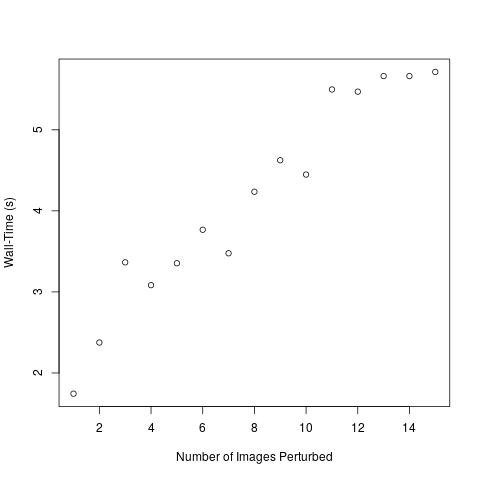
\includegraphics[scale = 0.7]{WallTimeConstant.jpg}
    \caption{Plot of Wall Time vs. Images Analyzed}
    \label{fig:my_label}
\end{figure}

The relationship appears to be roughly linear as expected, and the mean processing time per image was calculated to be 0.686 seconds.

\subsubsection{Yellow - Green Pixel Shift}
Similar to the last algorithm, this one uses a single loop to iterate and modify the images. It make the execution time linear and it makes the algorithm O(n). 
\begin{figure}[H]
\centering
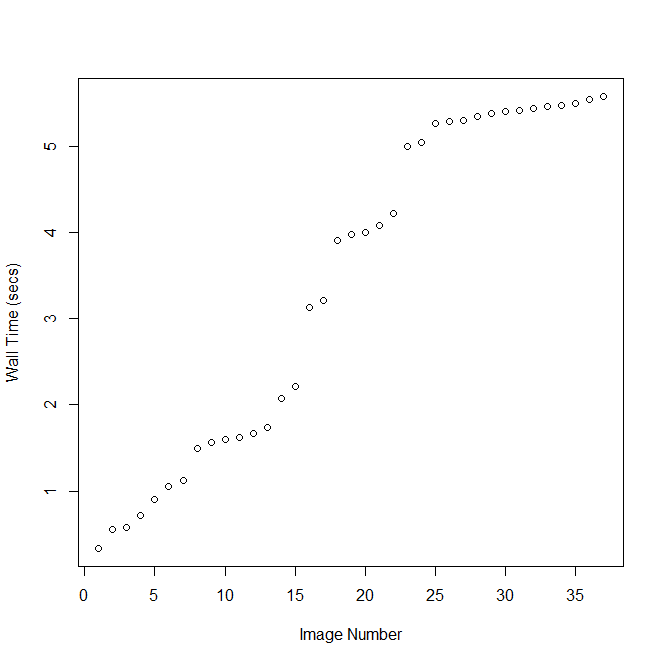
\includegraphics[scale = 0.4]{Walltime_shift_2.png}
    \caption{Plot of Wall Time vs. Images Analyzed}
    \label{fig:my_label}
\end{figure}
The wall-times for this algorithm are relatively short. The output is roughly linear, but there are pictures that are taking longer time to process.
\subsubsection{CCP Attack}
The runtime complexity of the CCP Attack algorithm will likely be O(N * M), where N is the number of images being processed and M is the size of the image. An O(N * M) time complexity means that the algorithm's running time grows linearly with the product of the input sizes N and M. This implies that as the input size increases, the time taken to execute the algorithm will increase proportionally. 
\subsubsection{Image Overlay}


\subsection{Appendix C: Performance}
\subsubsection{RGB Pixel Swap}
Because I was unable to run my code for a majority of the time, I was unable to generate the type error. We should be focused on type II error, leaving only a part of the matrix applicable. I was not able to determine the number of images for which the classifier was fooled. 

\subsubsection{Square Contrasting Color Overlay}
To measure the performance of the algorithm, the model was used to predict the class of all dandelion and grass images, and type II error was recorded. Typically, classification error data is presented in a confusion matrix, but since we are only concerned with type II error, when the image is mis-classified, only part of the matrix is relevant. This algorithm was only able to fool the classifier for 6 dandelion images (16.22\%) while changing only 1\% of pixels. .

\subsubsection{Yellow - Green Pixel Shift}
As for the performance of the Yellow - Green Pixel Shift, similar to the last algorithm, if we only concerned about the type II error, the algorithm is able to fool 9 dandelion images (24.32\%), by changing 1\% pixels. None of the grass images are fooled.  

\subsubsection{CCP Attack}
The performance of a Color Channel Perturbation attack can be evaluated by a number of metrics. One of the most common metrics to evaluate the performance is simply accuracy. Accuracy measures the percentage of correctly classified images out of the total number of images in the test set. To evaluate accuracy of a CCP attack, one can compute the accuracy of the target model on the perturbed test image and compare it to the accuracy of the original test image. Without this attack properly functioning, it is difficult to determine how many dandelion images and grass images were successfully fooled. However, through research and the multiple attempts at a functioning CCP Attack, the predicted performance of this algorithm is such that it should be able to fool 5 dandelion images (13.15\%) and 8 grass images (16.32\%) by changing 1\% of pixels.  

\subsubsection{Image Overlay}
The performance of this algorithm would have been assessed via the model. By factoring in the images it was able to fool over the total number of images to get a success rate percentage. However, as the algorithm did not function properly we could not generate the metrics. 

\subsection{Appendix D: Justification/Announcement Allocation}
\subsubsection{RGB Pixel Swap}
This sub algorithm is a simple change of pixels in each image. This algorithm selected pixel based on color and change them according to the commands. At least, that is what it is intended to do. I chose to use a semi-basic function to cut down on run-time and in doing this, I sacrificed some of the performance. However, because of our other algorithms, I think this was a good choice. Many of our algorithms are much more complex and maximize on performance. They were not super fast though. This led me to believe we needed a simple but quick algorithm that would process some of the images. The testing pairs for this algorithm are the dandelion and grass files run through the 'random' function to modify them before being sent though the model. They are then saved to the grass directory. There, they are paired with their original images to form the testing pairs. For this algorithm, there were a lot of knowledge representations required. For example, the user needs knowledge of the desired libraries, functions, and packages used in the code. The user also needs knowledge of image processing and alteration by way of reshaping arrays, modifying color channels, and converting between representations of images and arrays. 


\subsubsection{Square Contrasting Color Overlay}
This algorithm functions as a simple attack for images that have a high concentration of identifiable pixels at the center. This is in contrast to the other algorithms used, which tend to select pixels by color or intensity rather than location. Additionally, the algorithm was simple to implement and understand, which was an issue with prior attempts. Originally I attempted the Fast Gradient Sign Method, which calculates the gradient of the decision boundary and perturbs pixels against the gradient. Typically, the perturbations would be done such that they are along the gradient of the nearest class, but in the case of a binary classifier, it is simply against the gradient of the original class since there are only two classes. Although the algorithm ran and computed a gradient, it was always on the edge of an image, and almost never led to mis-classification. This was likely due to errors in the dimensions and data types used throughout the function, as that was a frequent issue I ran into while attempting the algorithm. Specifically, the Tensorflow documentation contained functions in python that I was having difficulty finding an R equivalent for, and reticulate seemed to throw errors when used. This led to using the Contrasting Color Overlay instead due to the ease of implementation, but the original attempt at FGSM is viewable in the repository under the "KevinBraner-FGSM" branch.


\subsubsection{Yellow - Green Pixel Shift}
This algorithm changes the 1\% highest red pixels to blue when fooling dandelion pictures, and it does the opposite for the grass pictures. 
\\
\\
The result for the algorithm did not go as well as we expected. And the result that no grass image is fool is because of the fact that, even if there are green areas on the grass that is replaced by yellow, the yellow areas mostly appear on the tips of the grass, or even on the sky. Therefore, the yellow area will not be classified as dandelion flowers, but some random areas. This is the reason why it doesn't do well for grass pictures. 
\\
\\
However, there are cases that we should choose this algorithm. It's very simple and it takes a short amount of time to execute. The wall time for the total 37 pages is less than 6 seconds. Therefore, Yellow - Green Pixel shift will be a good choice when dealing with a large amount of pictures. And it works relatively well with dandelion images. (the highest success rate among all the working algorithm, 24.32\%). And this algorithm should work a lot better if given a bigger pixel budget. given 5\% or more pixel budget, the green pixels will cover the whole flower, which will lead to a much higher success rate. 
\\
\\
As for the run-time and performance trade-offs, the algorithm will rescale the image to 224*224 to shorten the run-time. However, it should not affect the performance since the model resize the original picture into the 224*224, and by doing that ahead of time, we will have better control over the pixel budget. 

\subsubsection{CCP Attack}

The Color Channel Perturbation Attack utilizes the Convoluted Neural Network model to fool a binary image classifier. CNNs are designed to recognize patterns and features in input images and learn to classify them into different categories. Like any machine learning model, CNNs have performance tradeoffs which must be taken into consideration. In the context of this project, the most impactful tradeoff that needed to be accounted for was the interpretability. It can be challenging to understand how the model is making predictions and which features its relying on. By attacking the three primary color channels (RGB), the inerpretability of the algorithm is significantly improved. As per the walltime and performance of the algorithm, it is difficult to determine these aspects without a funcitoning algorithm. However, the algorithm 
\\

illustrate the design decisions you chose, why you chose them, and what you would have expected in terms of reasonable runtime/performance tradeoffs, as well as considerations such as how you would/should generate the testing pairs for the machine learning algorithms, what knowledge representations you think are sufficient 


\subsubsection{Image Overlay}

In the initial steps of devising this algorithm a Carlini and Wagner adversarial attack was . In theory, it will slightly perturb an image using an optimization framework to cause a higher degree of miss-classification within the model. That proved a little challenging and lead to a change of course to the Image Overlay approach. Using a similar thought process to the Carlini and Wagner attack, the transparent image would perturb the initial image to confuse the model by placing an incorrect image over the original.

As for run-time and performance trade-offs, image re-scaled was used to speed up algorithm performance due to the amount of images being processed. Obviously as the number of images increases so will run-time and with that the complexity of the implementation within the model. The thought process was that a more rudimentary algorithm such as Image Overlay would not only be easier to implement but also a faster running algorithm.

Image Overlay was designed with testing in mind. The algorithm creates an output path unless specified within the code to show the results prior to enterring in the model. 




illustrate the design decisions you chose, why you chose them, and what you would have expected in terms of reasonable runtime/performance tradeoffs, as well as considerations such as how you would/should generate the testing pairs for the machine learning algorithms, what knowledge representations you think are sufficient 

\end{document}